\documentclass[10pt]{beamer}

\usetheme{Berkeley}

\usepackage[utf8]{inputenc}
\usepackage[slovene]{babel}

\usepackage{amsmath, amssymb}

\usepackage{tikz}
\usetikzlibrary{math}
\usetikzlibrary{decorations.fractals}
\usetikzlibrary{lindenmayersystems}

\usepackage{graphicx}

\usepackage{pgfplots}
\pgfplotsset{compat=1.18}

% Standardne množice
\newcommand{\NN}{\mathbb{N}}
\newcommand{\ZZ}{\mathbb{Z}}
\newcommand{\QQ}{\mathbb{Q}}
\newcommand{\RR}{\mathbb{R}}
\newcommand{\CC}{\mathbb{C}}
\newcommand{\FF}{\mathbb{F}}

%%% Quantifiers
\newcommand{\all}[1]{\forall #1 \,.\,}
\newcommand{\some}[1]{\exists #1 \,.\,}
\newcommand{\exactlyone}[1]{\exists! #1 \,.\,}

% Implikacija
\newcommand{\lthen}{\Rightarrow}
\newcommand{\liff}{\Leftrightarrow}

%%% Množice
\newcommand{\set}[1]{\left\{#1\right\}}
\newcommand{\setb}[2]{\set{#1 \ | \  #2}}

%% Preslikave
\newcommand{\img}[1]{#1_{*}}
\newcommand{\invimg}[1]{#1^{*}}
\newcommand{\lin}[1]{\mathcal{#1}}

%% Odvod
\newcommand{\podv}[2]{\frac{\partial #1}{\partial #2}}

%% Metrični prostori
\newcommand{\norm}[1]{||#1||}

\DeclareMathOperator{\grad}{grad}




\title[Fraktalne dimenzije]{Fraktalne dimenzije}
\author{Ruslan Urazbakhtin}
\institute{Fakulteta za matematiko in fiziko, Univerza v Ljubljani}
\date{6.\ maj 2025}

\begin{document}

\begin{frame}
  \titlepage

  \vfill % Отодвигает цитату вниз

  \begin{flushright}
    \small
    \textit{"`Much of the beauty of fractals is to be found in their mathematics"'} \\
    \hspace{1em} --- Kenneth Falconer
  \end{flushright}
\end{frame}

\begin{frame}{Kazalo}
  \tableofcontents
\end{frame}

\section{Uvod}
\subsection{Kaj so fraktali?}

\begin{frame}{Kaj so fraktali?}
    \centering
    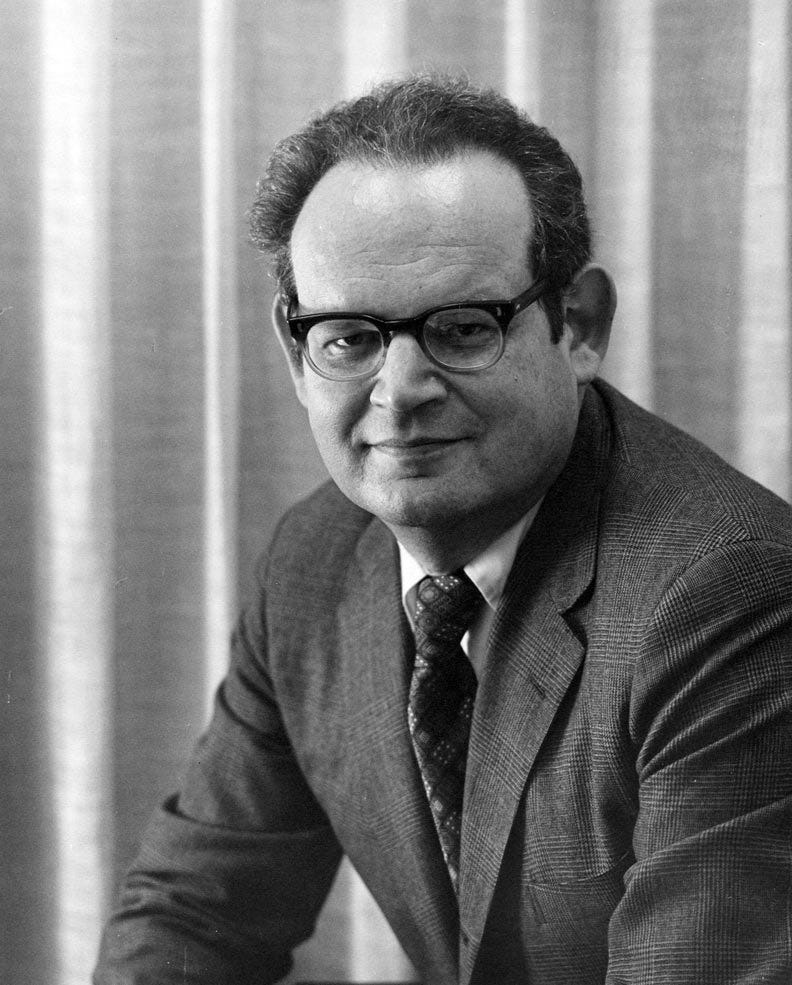
\includegraphics[width=0.5\textwidth]{img/mandelbrot.jpg} 
\end{frame}

\begin{frame}{Kaj so fraktali?}
    \begin{itemize}
        \item Besedo "`fraktal"' je uvedel matematik Benoit Mandelbrot v svojem temeljnem eseju leta 1975. Izvira iz latinske besede "`fractus"'. 
        \item Besedo "`fraktal"' Mandelbrot je uporabljal za opis patoloških množic, ki niso bili usklajene z običajno evklidsko geometrijo.
        \item V svojem originalnem eseju Benoit Mandelbrot je definiral fraktal kot množico, ki ima Hausdorffovo dimenzijo strogo večjo od njene topološke dimenzije. 
    \end{itemize}    
\end{frame}

\begin{frame}{Kaj so fraktali?}
    Če rečemo, da je neka množica \(F\) fraktal, potem si mislimo, da
    \begin{enumerate}
        \item \(F\) ima fino strukturo, tj.\ podrobnosti se vidijo vedno enako (neodvisno od skale);
        \item \(F\) je dovolj nenaravna, da je ne moremo opisat s pomocjo elementarne geometrije tako lokalno kot globalno;
        \item \(F\) včasih ima samopodobno obliko;
        \item Običajno je fraktalna dimenzija \(F\) večja od njene topološke dimenzije;
        \item V večini primerov  je \(F\) definirana na zelo preprost način, običajno rekurzivno.
    \end{enumerate}   
\end{frame}

\begin{frame}{Zakaj potrebujemo fraktalno dimenzijo?}
    \begin{itemize}
        \item Metode iz evklidske geometrije/analize niso dovolj, da opišemo lastnosti fraktalov.
        \item Fraktalna geometrija nam ponuja osnovno konstrukcijo za obravnavo množic, ki izgledajo nekako nenaravno.
        \item Zelo na grobo povedano nam dimenzija množice pove, koliko prostora ta zavzema v ambientnem prostoru. 
        \item Dimenzija meri kompleksnost množice na poljubno majhnih skalah ter opisuje nekatere njene geometrijske in topološke lastnosti.
    \end{itemize}    
\end{frame}

% Скрыть
% \subsection{Opomba o teorije mere}
% \begin{frame}{Mera}
%     \begin{itemize}
%         \item Če želimo govoriti o fraktalnih dimenzijah, moramo poznati osnovne ideje teorije mere.
%         \item Bomo obravnavali le mere na \(\R^n\).
%     \end{itemize}    
% \end{frame}

\begin{frame}{Borelova \(\sigma\)-algebra}
    \begin{definicija} 
        Družina podmnožic \(\Sigma\) množice \(\R^n\) je \emph{\(\sigma\)-algebra}, če:
        \begin{enumerate}
            \item \(\R^n \in \Sigma\);
            \item Če je \(A \in \Sigma\), potem \(A^c \in \Sigma\);
            \item Poljubna števna unija množic iz \(\Sigma\) je element \(\Sigma\).
        \end{enumerate} 
    \end{definicija}

    \pause

    \begin{definicija} \ 
        \begin{itemize}
            \item Najmanjšo \(\sigma\)-algebro na \(\R^n\), ki vsebuje vse odprte podmnožice \(\R^n\), imenujemo \emph{Borelova \(\sigma\)-algebra}.
            \item Podmnožica \(A \subseteq \R^n\) je \emph{Borelova}, če pripada Borelovi \(\sigma\)-algebri.
        \end{itemize}
    \end{definicija}
\end{frame}

\begin{frame}{Borelova \(\sigma\)-algebra}
    \begin{definicija} \ 
        \begin{itemize}
            \item Najmanjšo \(\sigma\)-algebro na \(\R^n\), ki vsebuje vse odprte podmnožice \(\R^n\), imenujemo \emph{Borelova \(\sigma\)-algebra}.
            \item Podmnožica \(A \subseteq \R^n\) je \emph{Borelova}, če pripada Borelovi \(\sigma\)-algebri.
        \end{itemize}
    \end{definicija}

    \begin{opomba}
        \begin{itemize}
            \item Vse odprte in vse zaprte množice so Borelovi.
            \item Poljubna števna unija (presek) odprtih (zaprtih) množic je Borelova množica. 
            \item Vsi množici, ki smo jih bomo obravnavali, bodo Borelovi.
        \end{itemize}
    \end{opomba}
\end{frame}

\begin{frame}{Mera na \(\R^n\)}
    \begin{definicija}
        Preslikava \(\mu: \mathcal{P}(\R^n) \to [0, \infty) \cup \set{\infty}\) je \emph{mera} na \(\R^n\), če 
        \begin{enumerate}
            \item \(\mu(\emptyset) = 0\);
            \item Če je \(A \subseteq B\), potem \(\mu(A) \leq \mu(B)\);
            \item Če je \(\set{A_i}_{i \in \N}\) števna družina podmnožic \(\R^n\), potem 
            \[\mu\left(\bigcup_{i=1}^\infty A_i\right) \leq \sum_{i=1}^{\infty} \mu (A_i)\]
            \item Če je \(\set{A_i}_{i \in \N}\) števna družina paroma disjunktnih Borelovih podmnožic \(\R^n\), potem 
            \[\mu\left(\bigcup_{i=1}^\infty A_i\right) = \sum_{i=1}^{\infty} \mu (A_i)\]
        \end{enumerate}
    \end{definicija}
\end{frame}

\begin{frame}{Mera na \(\R^n\)}
    \begin{definicija}
            Pravimo tudi, da je \(\mu(A)\) \emph{mera množice \(A\)}.
    \end{definicija}

    \begin{opomba} \
        \begin{itemize}
            \item \(\mu(A)\) lahko si predstavljamo kot "`velikost"' množice \(A\), ki je izmerjena na nek način.
            \item 4.\ pogoj pravi, da če množico \(A\) razbijemo na števno mnogo paroma disjunktnih Borelovih množic, potem vsota mer delov je enaka mere celotne množice (ponavadi ga težko dokazati).
        \end{itemize}
    \end{opomba}
\end{frame}

\begin{frame}{Primeri mer}
    \begin{itemize}
        \item \textbf{Mera štetja.}
        
        Naj bo \(A \subseteq \R^n\). Definiramo \(\mu(A) = \begin{cases}
            n; &|A| = n \in \N, \\ \infty; &\text{sicer}
        \end{cases}\).
        
        Potem \(\mu\) je mera na \(\R^n\).
        \item \textbf{Točkasta masa.}
        
        Naj bo \(a \in \R^n, \ A \subseteq \R^n\). Definiramo \(\mu(A) = \begin{cases}
            1; &a \in A, \\ 0; &\text{sicer}
        \end{cases}\).
    
        Potem \(\mu\) je mera (porazdelitev mase) na \(\R^n\).
    \end{itemize}
\end{frame}

\begin{frame}[t]{Lebesgueva \(\mathcal{L}^n\) mera}
    \only<1>{Lebesgueva \(\mathcal{L}^n\) mera na \(\R^n\) je posplošitev evklidskih pojmov "`dolžina"', "`ploščina"', "`volumen"' itn.\  na večji razred množic.}

    \only<2>{
        Naj bo \(A = \setb{(x_1, \ldots, x_n) \in \R^n}{ a_i \leq x_i \leq b_i}\) kvader v \(\R^n\), potem \(n\)-dim volumen množice \(A\) je \[\text{vol}^n(A) := (b_1 - a_1)(b_2-a_2)\ldots(b_n - a_n).\]
        \begin{definicija}
            \emph{Lebesgueva mera \(\mathcal{L}^n: \mathcal{P}(\R^n) \to [0, \infty]\)} je definirana s predpisom
            \[\mathcal{L}^n(A) = \inf \setb{\sum_{i=1}^{\infty} \text{vol}^n(A_i) }{A \subseteq \bigcup_{i =1}^\infty A_i},\]
            kjer so \(A_i\) kvadri.
        \end{definicija}  
    }
\end{frame}

% Скрыть
% \begin{frame}{Lebesgueva \(\mathcal{L}^n\) mera}
%     \begin{opomba} \
%         \begin{itemize}
%             \item Gledamo vsa pokritja množice \(A\) z kvadri in vzemimo najmanjši možen volumen.
%             \item \(\mathcal{L}^1\) je posplošitev pojma "`dolžina"', \(\mathcal{L}^2\) je posplošitev pojma "`ploščina"' itn.
%         \end{itemize}            
%     \end{opomba}  
% \end{frame}

\begin{frame}[t]{Cantorjeva množica \(C\)}
    Izračunamo dolžino \(\mathcal{L}^1(C)\) Cantorjeve množice \(C  = \bigcup_{n=1}^\infty C_n\).

    \begin{center}
        \drawCantor{5}
    \end{center}  

    \begin{lema}
        Naj bosta \(A, B \subseteq \R^n\) Borelovi, \(A \subseteq B\). Naj bo \(\mu\) mera na~\(\R^n\). \\ Potem \(\mu(B \setminus A) = \mu(B) - \mu(A)\).
    \end{lema}
\end{frame}

\begin{frame}[t]{Kochova krivulja \(K\)}
    \begin{center}
        \drawKoch
    \end{center}    
\end{frame}

\subsection{Podobnostna dimenzija}

\begin{frame}[t]{Kaj je narobe z \(C\) in \(K\)?}
    \pause
    \begin{itemize}
        \item Očitno je, da je pri izbiri dimenzije nekaj narobe (torej z nami). 
        \item Ni možnosti, da bi dobili kaj pametnega, če bi računali ploščino daljice ali šteli njene točke.
    \end{itemize}  
\end{frame}

\begin{frame}[t]{Ali obstaja boljša možnost za izbiro dimenzije?}
    \pause
    Obstaja.
\end{frame}

\begin{frame}[t]{Podobnostna dimenzija}
    \begin{itemize}
        \item Kaj lahko povemo o masi daljice, če dvakrat zmanjšamo njeno dolžino?
        \item Kaj lahko povemo o masi kvadrata, če dvakrat zmanjšamo dolžino njegove stranice?
    \end{itemize}
    \pause
    Torej \[m(\lambda D) = \lambda^s m(D).\]
\end{frame}

\begin{frame}[t]{Podobnostna dimenzija}
    Torej \[m(\lambda D) = \lambda^s m(D).\]
    Kaj se zgodi z maso Cantorjeve množice, če trikrat zmanjšamo začetni interval?
    \begin{center}
        \drawCantor{5}
    \end{center}   
    
\end{frame}

\begin{frame}[t]{Podobnostna dimenzija}
    Kaj se zgodi z maso Kochove krivulje, če trikrat zmanjšamo začetni interval?
    \begin{center}
        \drawKoch
    \end{center}       
\end{frame}

\begin{frame}[t]{Podobnostna dimenzija}
    \begin{definicija}
        Naj bo množica \(F \subseteq \R^n\) sestavljena iz \(m\) kopij same sebe, kjer je vsaka kopija zmanjšana za faktor \(r\). Potem rečemo, da ima množica~\(F\) \emph{podobnastno dimenzijo} enako \(\log_r m\).
    \end{definicija}  
    \pause
    Spet imamo en problem... 
    
    \pause
    Samopodobnih množic je zelo malo. Recimo, že krožnica ni taka.

    \begin{center}
        \drawSmile
    \end{center}    
\end{frame}

\begin{frame}[t]{Podobnostna dimenzija}
    \begin{definicija}
        Naj bo množica \(F \subseteq \R^n\) sestavljena iz \(m\) kopij same sebe, kjer je vsaka kopija zmanjšana za faktor \(r\). Potem rečemo, da ima množica~\(F\) \emph{podobnastno dimenzijo} enako \(\log_r m\).
    \end{definicija}  
    Spet imamo en problem... 
    
    Samopodobnih množic je zelo malo. Recimo, že krožnica ni taka.

    \begin{center}
        \drawSmileFunny
    \end{center}    
\end{frame}

\section{Hausdorffova dimenzija}
\begin{frame}{Hausdorffova dimenzija}
    \begin{itemize}
        \item Hausdorffova dimenzija izmed vseh "`fraktalnih"' dimenzij, ki jih ljudje uporabljajo, je najbolj stara in verjetno najbolj pomembna. 
        \item Lahko jo definiramo za poljubno množico in matematično je zelo priročna, ker je osnovana na meri, s katero lahko relativno preprosto kaj naredimo.
        \item Glavna pomanjkljivost je, da jo v večini situacij težko izračunati ali oceniti z numerični metodi.
    \end{itemize}
\end{frame}

\subsection{Hausdorffova mera}
\begin{frame}[t]{Hausdorffova mera}
    \only<1> {
        \begin{definicija}
            Naj bo \(F \subseteq \R^n\). Naj bo \(\set{U_i}\) števna družina množic iz \(\R^n\), za katero velja:
            \begin{enumerate}
                \item \(\all{i \in \N} 0 \leq |U_i| \leq \delta\);
                \item \(F \subseteq \bigcup_{i=1}^\infty U_i\).
            \end{enumerate}
            Potem \(\set{U_i}\) imenujemo \emph{\(\delta\)-pokritje} množice \(F\).
        \end{definicija}
    }
    \pause
    Naj bo \(F \subseteq \R^n\) in \(s \geq 0\). Za vsak \(\delta > 0\) definiramo 
    \[\mathcal{H}^s_\delta(F) = \inf \setb{\sum_{i=1}^{\infty}|U_i|^s}{\set{U_i} \ \text{je \(\delta\)-pokritje \(F\)}}\]
    %
    \pause
    Ko \(\delta \to 0\), razred možnih pokritij \(F\) se zmanjšuje, torej \(\inf\) narašča, torej lahko definiramo:
    \[\mathcal{H}^s(F) = \lim_{\delta \to 0} \mathcal{H}^s_\delta(F)\]
    Ta limita vedno obstaja za vsako množico \(F \subseteq \R^n\). 

    \pause    
    Število \(\mathcal{H}^s(F)\) imenujemo \emph{\(s\)-dim Hausdorffova mera} množice \(F\).

    \begin{trditev}
        \(\mathcal{H}^s\) je mera na \(\R^n\).
    \end{trditev}      
\end{frame}

\begin{frame}[t]{Hausdorffova mera}
    \begin{opomba}
        Hausdorffova mera je posplošitev Lebesgueve mere na necele dimenzije. Se da pokazati, da 
        \[\mathcal{H}^n(F) = \frac{1}{c_n} \mathcal{L}^n(F),\]
        kjer je \(c_n\) volumen \(n\)-dim krogle z polmerom \(\frac{1}{2}\), tj. 
        \[c_n = \frac{\pi^{(n/2)}}{\Gamma(n/2 + 1)} \left(\frac{1}{2}\right)^n\]
    \end{opomba}  
\end{frame}

\begin{frame}[t]{Lastnosti skaliranja}
    \only<1> {
        \begin{definicija}
            \emph{Podobnostna preslikava} z koeficientom podobnosti \(c > 0\) je preslikava \(P: \R^n \to \R^n\), za katero velja:
            \[\all{x, y \in \R^n} |P(x) - P(y)| = c|x-y|\]
        \end{definicija}
    }
    \pause
    Naj bo \(P: \R^n \to \R^n\) podobnostna preslikava z podobnostnim koeficientom \(c > 0\). Naj bo \(F \subseteq \R^n\).
    
    \only<2> {
        Dobro poznamo lastnosti skaliranja dolžine, ploščine, volumna, npr.
        \begin{itemize}
            \item \(\mathcal{L}^1(\img{P}(F)) = c \mathcal{L}^1(F)\)
            \item \(\mathcal{L}^2(\img{P}(F)) = c^2 \mathcal{L}^2(F)\)
            \item \(\mathcal{L}^3(\img{P}(F)) = c^3 \mathcal{L}^3(F)\)
        \end{itemize}
        Ali velja enako tudi za \(\mathcal{H}^s\)?
    }
    \pause
    \begin{trditev}
        \[\mathcal{H}^s(\img{P}(F)) = c^s \mathcal{H}^s(F)\]
    \end{trditev}   
\end{frame}

% \begin{frame}[t]{Lastnosti skaliranja}
%     \only<1> {
%         \begin{definicija}
%             \emph{Podobnostna preslikava} z koeficientom podobnosti \(c > 0\) je preslikava \(P: \R^n \to \R^n\), za katero velja:
%             \[\all{x, y \in \R^n} |P(x) - P(y)| = c|x-y|\]
%         \end{definicija}
%     }
%     \pause
%     Naj bo \(P: \R^n \to \R^n\) podobnostna preslikava z podobnostnim koeficientom \(c > 0\). Naj bo \(F \subseteq \R^n\).
    
%     \only<2> {
%         Dobro poznamo lastnosti skaliranja dolžine, ploščine, volumna, npr.
%         \begin{itemize}
%             \item \(\mathcal{L}^1(\img{P}(F)) = c \mathcal{L}^1(F)\)
%             \item \(\mathcal{L}^2(\img{P}(F)) = c^2 \mathcal{L}^2(F)\)
%             \item \(\mathcal{L}^3(\img{P}(F)) = c^3 \mathcal{L}^3(F)\)
%         \end{itemize}
%         Ali velja enako tudi za \(\mathcal{H}^s\)?
%     }
%     \pause
%     \begin{trditev}
%         \[\mathcal{H}^s(\img{P}(F)) = c^s \mathcal{H}^s(F)\]
%     \end{trditev}   
% \end{frame}

\begin{frame}[t]{Lastnosti skaliranja}
    \begin{definicija} Naj bosta \(X \subseteq \R^n\) in \(Y \subseteq \R^m\).
        Preslikava \(f: X \to Y\) je \emph{Höldorjeva} stopnje \(\alpha > 0\), če
        \[\some{c > 0} \all{x, y \in X} |f(x) -f(y)| \leq c|x-y|^\alpha\]             
    \end{definicija}  
    \pause
    \begin{trditev}
        Naj bo \(F \subseteq \R^n\) in \(f: F \to \R^n\) Höldorjeva preslikava stopnje \(\alpha > 0\). Potem za vsak \(s \geq 0\) velja:
        \[\mathcal{H}^{s/\alpha}(\img{f}(F)) \leq c^{s/\alpha} \mathcal{H}^s(F)\]
    \end{trditev}
\end{frame}

\begin{frame}[t]{Lastnosti skaliranja}
    \begin{trditev}
        Naj bo \(F \subseteq \R^n\) in \(f: F \to \R^n\) Höldorjeva preslikava stopnje \(\alpha > 0\). Potem za vsak \(s \geq 0\) velja:
        \[\mathcal{H}^{s/\alpha}(\img{f}(F)) \leq c^{s/\alpha} \mathcal{H}^s(F)\]
    \end{trditev}

    \begin{posledica}
        Če je \(f: F \to \R^n\) Lipschitzova, tj.
        \[\some{c > 0} \all{x, y \in X} |f(x) -f(y)| \leq c|x-y|,\]
        potem
        \[\mathcal{H}^{s}(\img{f}(F)) \leq c^{s} \mathcal{H}^s(F)\]
    \end{posledica}
\end{frame}

\subsection{Hausdorffova dimenzija}
\begin{frame}[t]{Hausdorffova dimenzija}
    Naj bo \(F \subseteq \R^n\). Gledamo funkcijo 
    \begin{align*}
        \mathcal{H}_F: [0, \infty) &\longrightarrow [0, \infty] \\
        s &\longmapsto \mathcal{H}^{s}(F)
    \end{align*}

    \begin{lema}
        Naj bo \(F \subseteq \R^n\). Če je \(\mathcal{H}^{s}(F) < \infty\), potem \(\mathcal{H}^{t}(F) = 0\) za vse \(t > s\).
    \end{lema}
\end{frame}

\begin{frame}[t]{Hausdorffova dimenzija}
    \begin{lema}
        Naj bo \(F \subseteq \R^n\). Če je \(\mathcal{H}^{s}(F) < \infty\), potem \(\mathcal{H}^{t}(F) = 0\) za vse \(t > s\).
    \end{lema}

    Oglejmo si graf funkcije \(\mathcal{H}_F\):
    \begin{center}
        \scalebox{0.8}{
            \drawGraf
        }        
    \end{center}    
\end{frame}

\begin{frame}[t]{Hausdorffova dimenzija}
    \begin{definicija}
        \emph{Hausdorffova dimenzija} množice \(F \subseteq \R^n\) je 
        \[\text{dim}_H F = \inf \setb{s \geq 0}{\mathcal{H}^{s}(F) = 0} = \sup \setb{s \geq 0}{\mathcal{H}^{s}(F) = \infty}\]
    \end{definicija} 

    \pause
    \only<2> {
        \begin{opomba}
            \begin{itemize}
                \item Po dogovoru \(\sup (\emptyset) = 0\).
                \item Ta dimenzija je definirana za poljubno podmnožico \(\R^n\).
            \end{itemize}   
        \end{opomba}
    }
    \pause 
    Imamo:
    \[
        \mathcal{H}^{s}(F) = \begin{cases}
            \infty; &0 \leq s < \text{dim}_H F \\ 
            0; &s > \text{dim}_H F;
        \end{cases}
    \]
    %
    Če je \(s = \text{dim}_H F\), potem \(\mathcal{H}^{s}(F)\) lahko \(0, \  \infty\) ali \(a \in \R\).    
\end{frame}

\begin{frame}[t]{Hausdorffova dimenzija krogle \(B^n\)}
    \begin{lema}
        \[\text{dim}_H B^n = n\]
    \end{lema}
    
    \pause
    Spomnimo se
    \begin{lema}
        \[\mathcal{H}^n(F) = \frac{1}{c_n} \mathcal{L}^n(F),\]
        kjer je \(c_n\) volumen \(n\)-dim krogle z polmerom \(\frac{1}{2}\), tj. 
        \[c_n = \frac{\pi^{(n/2)}}{\Gamma(n/2 + 1)} \left(\frac{1}{2}\right)^n\]
    \end{lema}
\end{frame}

\subsection{Lastnosti Hausdorffove dimenzije}
\begin{frame}[t]{Lastnosti Hausdorffove dimenzije}
    \begin{itemize}
        \item[(1)] \textbf{Monotonost.} Če je \(E \subseteq F\), potem \(\text{dim}_H E \leq \text{dim}_H F\).
        \pause
        \item[(2)] \textbf{Števna stabilnost.} Če je \(F_1, F_2, \ldots\) števno zaporedje množic, potem 
        \[\text{dim}_H \bigcup_{i=1}^\infty F_i = \sup_{1 \leq i < \infty} (\text{dim}_H F_i)\]
        \pause
        \item[(3)] \textbf{Dimenzija števnih množic.} Če je \(F\) števna, potem \(\text{dim}_H F = 0\).
        \pause
        \item[(4)] \textbf{Dimenzija odprtih množic.} Naj bo \(F \subseteq \R^n\) odprta podmnožica. Potem \(\text{dim}_H F = n\).
        \pause
        \item[(5)] \textbf{Dimenzija gladkih podmnogoterosti.} Naj bo \(F \subseteq \R^n\) gladka podmnogoterost dimenzije \(m\), potem \(\text{dim}_H F = m\). Posebej:
        \begin{itemize}
            \item Če je \(F\) gladka krivulja, potem \(\text{dim}_H F = 1\);
            \item Če je \(F\) gladka ploskev, potem \(\text{dim}_H F = 2\).
        \end{itemize}
    \end{itemize}
\end{frame}

% Скрыть
% \begin{frame}[t]{Lastnosti Hausdorffove dimenzije}
%     \begin{opomba}
%         To so osnovne lastnosti, ki jih lahko zahtevamo od dimenzije, če želimo, da je ta res posplošitev običajne evklidske dimenzije.
%     \end{opomba}
% \end{frame}

\begin{frame}[t]{Transformacijeske lastnosti Hausdorffove dimenzije}
    \begin{trditev}
        Naj bo \(F \subseteq \R^n\) in \(f: F \to \R^n\) Höldorjeva preslikava stopnje \(\alpha > 0\). Potem 
        \[\text{dim}_H \img{f}(F) \leq \frac{1}{\alpha} \text{dim}_H F\]        
    \end{trditev}
    \pause
    \only<2> {
        Spomnimo se
        \begin{trditev}
            Naj bo \(F \subseteq \R^n\) in \(f: F \to \R^n\) Höldorjeva preslikava stopnje \(\alpha > 0\). Potem za vsak \(s \geq 0\) velja:
            \[\mathcal{H}^{s/\alpha}(\img{f}(F)) \leq c^{s/\alpha} \mathcal{H}^s(F)\]
        \end{trditev}
    }
    \pause
    \begin{posledica}
        \ 
        \begin{itemize}
            \item Če je \(f: F \to \R^n\) Lipschitzova, potem \(\text{dim}_H \img{f}(F) \leq \text{dim}_H(F)\).
            \pause
            \item Če je \(f: F \to \R^n\) bi-Lipschitzova, tj.
            \[\some{c_1, c_2 > 0} \all{x, y \in X} c_1 |x- y| \leq |f(x) - f(y)| \leq c_2 |x - y|,\] 
            potem \(\text{dim}_H \img{f}(F) = \text{dim}_H(F)\).
        \end{itemize}
    \end{posledica}
\end{frame}

% Скрыть
% \begin{frame}[t]{Transformacijeske lastnosti Hausdorffove dimenzije}
%     \begin{opomba}
%         Posledica pove, da je \(\text{dim}_H\) invariantna glede na bi-Lipschitzeve preslikave. V posebnem, če sta množici imata različni Hausdorffovi dimenziji, potem ne obstaja bi-Lipschitzova preslikava med njima.
%     \end{opomba}
% \end{frame}

\begin{frame}[t]{Topološke lastnosti Hausdorffove dimenzije}
    \begin{trditev}
        Naj bo \(F \subseteq \R^n\). Če je \(\text{dim}_H F < 1\), potem je \(F\) \only<1>{...}\pause popolnoma nepovezana.
    \end{trditev}
\end{frame}

\subsection{Primeri računanja Hausdorffove dimenzije}
\begin{frame}[t]{Hausdorffova dimenzija Cantorjeva praha}
    \centering
    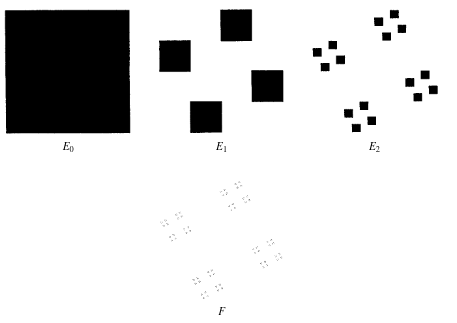
\includegraphics[width=\textwidth]{img/cantor_dust.png} 
\end{frame}

\begin{frame}[t]{Hausdorffova dimenzija Cantorjeve množice in Kochove krivulje}
    \begin{primer}
        Naj bo \(C\) Cantorjeva množica in \(K\) Kochova krivulja, potem
        \begin{itemize}
            \item \(\text{dim}_H C = \log_3 2 = 0.6309\ldots\)
            \item \(\text{dim}_H K = \log_3 4 = 1.2618\ldots\)
        \end{itemize}
    \end{primer}    
\end{frame}

\section{Škatlasta dimenzija}
\subsection{Ekvivalentne definicije}
\begin{frame}[t]{Druge vrste dimenzij}
    \begin{opomba}
        \begin{itemize}
            \item Hausdorffova dimenzija je osnova.
            \item Ni res, da vse definicije delujejo za vse množice.
            \item Osnovna ideja za vse dimenzije je "`meritev"' v skali \(\delta > 0\), tj. za vsak \(\delta > 0\) merimo množico na način, ki ignorira nepravilnosti, ki so manjše od \(\delta\). Nato pa gledamo, kaj se zgodi v limiti \(\delta \to 0\).
        \end{itemize}
    \end{opomba}
\end{frame}

\begin{frame}[t]{Škatlasta dimenzija}
    \only<1> {
        \begin{definicija}
            Naj bo \(f: \R_{>0} \to \R\) funkcija. 
            \begin{itemize}
                \item \emph{Spodnja limita} funkcije \(f\) ko gre x proti \(0\) je 
                \[\underline{\lim}_{x \to \infty} f(x) := \lim_{r \to 0} \left(\inf \setb{f(x)}{0< x < r}\right)\]
                \item \emph{Zgornja limita} funkcije \(f\) ko gre x proti \(0\) je 
                \[\overline{\lim}_{x \to \infty} f(x) := \lim_{r \to 0} \left(\sup \setb{f(x)}{0< x < r}\right)\]
            \end{itemize}
        \end{definicija}
    }

    \pause
    Naj bo \(F \subseteq \R^n\) omejena in neprazna. Označimo z \(N_\delta(F)\) najmanjšo število množic s premerom kvečjemu \(\delta>0\), ki jih potrebujemo za pokritje \(F\).
    
    \pause   
    \begin{definicija}
        \begin{itemize}
            \item \emph{Spodnja škatlasta dimenzija} množice \(F\) je 
            \[\underline{\text{dim}}_B F = \underline{\lim}_{\delta \to 0} \frac{\ln N_\delta(F)}{-\ln \delta}\]
            \item \emph{Zgornja škatlasta dimenzija} množice \(F\) je 
            \[\overline{\text{dim}}_B F = \overline{\lim}_{\delta \to 0} \frac{\ln N_\delta(F)}{-\ln \delta}\]
        \end{itemize}  
    \end{definicija}
\end{frame}

\begin{frame}[t]{Škatlasta dimenzija}  
    \begin{definicija}
        \begin{itemize}
            \item \emph{Spodnja škatlasta dimenzija} množice \(F\) je 
            \[\underline{\text{dim}}_B F = \underline{\lim}_{\delta \to 0} \frac{\ln N_\delta(F)}{-\ln \delta}\]
            \item \emph{Zgornja škatlasta dimenzija} množice \(F\) je 
            \[\overline{\text{dim}}_B F = \overline{\lim}_{\delta \to 0} \frac{\ln N_\delta(F)}{-\ln \delta}\]
            \item Če \(\underline{\text{dim}}_B F = \overline{\text{dim}}_B F\), potem skupno število imenujemo \emph{Škatlasta dimenzija} množice \(F\), tj. 
            \[\text{dim}_B F = \lim_{\delta \to 0} \frac{\ln N_\delta(F)}{-\ln \delta}\]
        \end{itemize}  
    \end{definicija}
\end{frame}

% Скрыть
% \begin{frame}[t]{Škatlasta dimenzija}  
%     \begin{opomba}
%         \begin{itemize}
%             \item Upoštevamo, da je \(\delta > 0\) dovolj majhen, da \(- \ln \delta > 0\).
%             \item Da nimamo težav \(\ln \infty\) ali \(\ln 0\), obravnavamo le omejeni neprazni množici.
%         \end{itemize}
%     \end{opomba}
% \end{frame}

\begin{frame}[t]{Škatlasta dimenzija (ekvivalentne oblike)}  
    \begin{definicija}
        Naj bo \(F \subseteq \R^n\) omejena in neprazna. \emph{Škatlasta dimenzija} množice~\(F\) je 
        \[\text{dim}_B F = \lim_{\delta \to 0} \frac{\ln N_\delta(F)}{-\ln \delta}\]
        kjer je \(N_\delta(F)\) lahko:
        \begin{itemize}
            \item najmanjše število množic s premerom kvečjemu \(\delta\), ki pokrivajo \(F\);
            \item najmanjše število zaprtih krogel z radijem \(\delta\), ki pokrivajo \(F\);
            \item najmanjše število zaprtih kvadrov s stranico \(\delta\), ki pokrivajo \(F\);
            \item število \(\delta\)-mreža kvadrov, ki sekajo \(F\);
            \item največje število disjunktnih zaprtih krogel z radijem \(\delta\) in središči na množici \(F\).
        \end{itemize}
    \end{definicija}
\end{frame}

% Скрыть
% \begin{frame}[t]{Škatlasta dimenzija (ekvivalentne oblike)}  
%     \begin{opomba}
%         \begin{itemize}
%             \item Lahko nadaljujemo ta seznam. V praksi izberimo najbolj relevanten za podano podmnožico.
%             \item V definiciji \(\delta \to 0\) lahko nadomestimo s poljubnim padajočim zaporedjem \(\delta_k\), za katero velja: 
%             \[\lim_{k \to \infty} \delta_k = 0\]
%         \end{itemize}
        
%     \end{opomba}
% \end{frame}

\begin{frame}[t]{\(\delta\)-mreža}  
    \[\text{dim}_B F = \lim_{\delta \to 0} \frac{\ln N_\delta(F)}{-\ln \delta}\]
    \begin{center}
        \scalebox{0.9}{
            \drawMesh
        }        
    \end{center}   
\end{frame}

\begin{frame}[t]{Disjunktne zaprte krogle}  
    \[\text{dim}_B F = \lim_{\delta \to 0} \frac{\ln N_\delta(F)}{-\ln \delta}\]
\end{frame}

\begin{frame}[t]{Škatlasta dimenzija Cantorjeve množice}  
    \begin{primer}
        Naj bo \(C\) Cantorjeva množica, potem 
        \[\text{dim}_H C = \log_3 2 = 0.6309\ldots\]
    \end{primer}
\end{frame}

\subsection{Relacija med Hausdorffovo in škatlasto dimenzijo}
\begin{frame}[t]{Relacija med Hausdorffovo in škatlasto dimenzijo}
    \begin{trditev}
        \[\text{dim}_H F \leq \underline{\text{dim}}_B F \leq \overline{\text{dim}}_B F\]
    \end{trditev}

    \pause
    \begin{opomba}
        V splošnem enakost NE velja, ne glede na to, da za nekatere lepe množice enakost drži.
    \end{opomba}
\end{frame}

\subsection{Lastnosti škatlaste dimenzije}
\begin{frame}[t]{Lastnosti škatlaste dimenzije}
    \begin{itemize}
        \item[(1)] \textbf{Monotonost.} \(\underline{\text{dim}}_B\) in \(\overline{\text{dim}}_B\) sta monotoni.
        \pause
        \item[(2)] \textbf{Končna stabilnost.} \(\overline{\text{dim}}_B\) je končno stabilna, tj. 
        \[\overline{\text{dim}}_B (E \cup F) = \max (\overline{\text{dim}}_B E, \overline{\text{dim}}_B F).\]
        Ta identiteta v splošnem NE velja za \(\underline{\text{dim}}_B\).
        \pause
        \item[(3)] \textbf{Dimenzija odprtih množic.} Naj bo \(F \subseteq \R^n\) odprta podmnožica. Potem \(\text{dim}_B F = n\).
        \pause
        \item[(4)] \textbf{Dimenzija gladkih podmnogoterosti.} Naj bo \(F \subseteq \R^n\) gladka podmnogoterost dimenzije \(m\), potem \(\text{dim}_B F = m\). 
    \end{itemize}
\end{frame}

\begin{frame}[t]{Težave škatlaste dimenzije}
    \begin{trditev}
        Naj bo \(F \subseteq \R^n\) omejena in neprazna. Velja:
        \begin{enumerate}
            \item \(\underline{\text{dim}}_B \Cl F = \underline{\text{dim}}_B F\).
            \item \(\overline{\text{dim}}_B \Cl F = \overline{\text{dim}}_B F\).
        \end{enumerate}
    \end{trditev}

    \pause
    \begin{posledica}
        V splošnem 
        \[\text{dim}_B \bigcup_{i=1}^\infty F_i \neq \sup_{1 \leq i < \infty} (\text{dim}_B F_i)\]
    \end{posledica}
\end{frame}

\begin{frame}[t]{Težave škatlaste dimenzije}
    Ali bomo še vedno imeli težave, če bomo gledali le zaprte množice?
    \pause

    \only<2> { Bomo... }
    
    \pause
    \begin{primer}
        Naj bo \(F = \setb{\frac{1}{n}}{n \in \N} \cup \set{0}\). 
        
        \(F\) je kompaktna množica z \(\text{dim}_B F = \frac{1}{2}\).
    \end{primer}
\end{frame}

\begin{frame}[t]{Od kod pride ta težava?}
    \begin{opomba}
        \begin{itemize}
            \item Pri računanju Hausdorffove dimenzije privzamemo, da množice pokritja \(\set{U_i}_{i \in \N}\) imajo različne velikosti.
            \item Pri računanju škatlaste dimenzije pa je velikost množic pokritja \(\set{U_i}_{1 \leq i \leq k}\) vedno fiksna (je enaka \(\delta\)).
            \pause
            \item Se nam zdi, da bi belo smiselno definirati mero 
            \[v(F) = \lim_{\delta \to 0} N_\delta(F) \delta^s\]
        \end{itemize}
    \end{opomba}
\end{frame}

\begin{frame}[t]{Povzetek o škatlasti dimenziji}
    \begin{itemize}
        \item Škatlasta dimenzija je zelo uporabna v praksi.
        \item Pogosto se da dokazati, da je enaka Hausdorffovi.
    \end{itemize}
\end{frame}

\begin{frame}
  \centering
  \Huge Hvala za pozornost!
\end{frame}

\end{document}
